\documentclass[tikz,border=3pt]{standalone}
\begin{document}
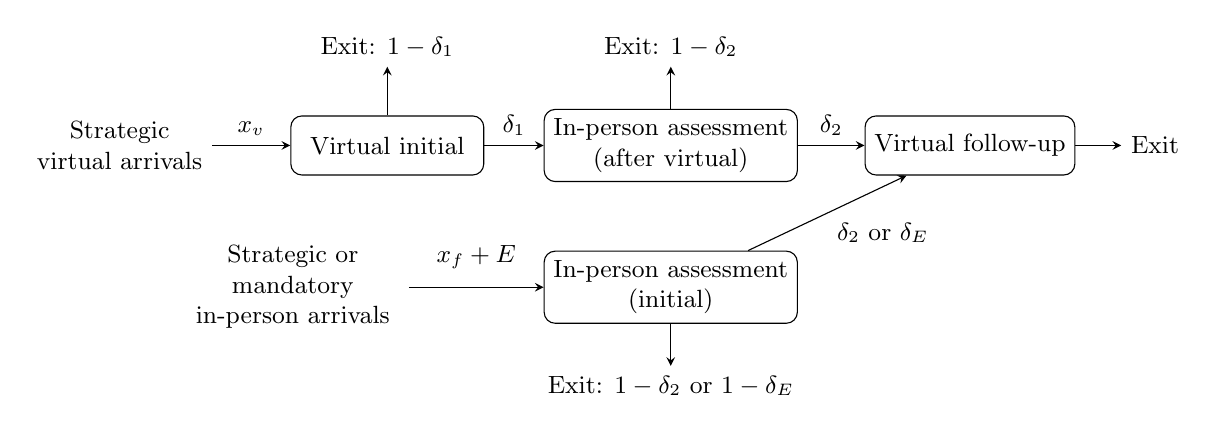
\begin{tikzpicture}[
    >=stealth,
    every node/.style={font=\small},
    box/.style={
        draw,
        rounded corners,
        align=center,
        minimum width=2.45cm,
        minimum height=.75cm
    }
]

\node[box] (v) at (0,1.6) {Virtual initial};

\node[box] (f) at (3.6,1.6)
    {In-person assessment\\(after virtual)};

\node[box] (r) at (7.4,1.6)
    {Virtual follow-up};

\node[box] (fi) at (3.6,-.2)
    {In-person assessment\\(initial)};

\node (out) at (9.75,1.6) {Exit};

\node[align=center,text width=2.1cm]
    (va) at (-3.4,1.6)
    {Strategic\\virtual arrivals};

\draw[->] (va)--node[above]{$x_v$}(v);

\draw[->] (v)--node[above]{$\delta_1$}(f);

\draw[->] (f)--node[above]{$\delta_2$}(r);

\draw[->] (fi)--node[below right]
    {$\delta_2$ or $\delta_E$}(r);

\draw[->] (r)--(out);

\draw[->] (v)--++(0,1)
    node[above]{Exit: $1-\delta_1$};

\draw[->] (f)--++(0,1)
    node[above]{Exit: $1-\delta_2$};

\draw[->] (fi)--++(0,-1)
    node[below]{Exit: $1-\delta_2$ or $1-\delta_E$};

\node[align=center,text width=2.7cm]
    (ia) at (-1.2,-.2)
    {Strategic or mandatory\\in-person arrivals};

\draw[->] (ia.east)--node[midway,above=3pt]
    {$x_f+E$}(fi.west);

\end{tikzpicture}
\end{document}
